\documentclass{article}
% \usepackage[margin=1in]{geometry}
\usepackage[brazil]{babel}
\usepackage[utf8]{inputenc}
\usepackage{amsmath}
\usepackage{indentfirst}
\usepackage{cite}
\usepackage{url}
\usepackage{graphics}
\usepackage{graphicx}
\usepackage{caption}
\usepackage{subcaption}
\usepackage{multirow}
\usepackage{amsfonts}

\title{Geração de Malhas\\{\large Trabalho 01}}
\author{Rafael Umino Nakanishi}

\date{}

\newcommand{\partials}[2]{
	\frac{\partial #1}{\partial #2}
}

\begin{document}
	\maketitle

	\section{Objetivo}
		O objetivo desse trabalho foi implentar o método de diferenças finitas para a Equação do calor (Eq. \ref{eq:calor}) para $t \geq 0$ e raio constante ($r=1$):

		\begin{eqnarray}
			\label{eq:calor}
			\frac{\partial u}{\partial t} = \Delta u
		\end{eqnarray}

		no domínio $\Omega = \{ (\theta,\phi): \pi/4 \leq \theta \leq \pi/2; 0 \leq \phi \leq 2\pi \}$ com as condições de contorno: 

		\begin{eqnarray*}
		\begin{cases}
			u(\pi/4, \phi, t) = 10\\
			u(\pi/2, \phi, t) = 0\\
			u(\theta, \phi, 0) = 1
		\end{cases}
		\end{eqnarray*}

	\section{Resolução do problema}
		\subsection{Laplaciano}
			Para a resolução do problema foi necessário realizar a discretização do Laplaciano para coordenadas esféricas:

			\begin{eqnarray}
				\label{eq:laplaciano}
				\Delta f = \frac{1}{\sqrt{g}} \frac{\partial}{\partial x^i} \bigg(\sqrt{g} g^{ij}\frac{\partial f}{\partial x^j}\bigg)
			\end{eqnarray}

			E desenvolvendo a Equação \ref{eq:laplaciano}, encontramos:

			\begin{eqnarray}
			 	\Delta f = \frac{1}{\rho^2} \partials{}{\rho}\bigg(\rho^2 \partials{f}{\rho}\bigg) + \frac{1}{\rho^2 \sin^2\phi}\partials{^2f}{\theta^2} + \frac{1}{\rho^2\sin\phi}\partials{}{\phi}\bigg(\sin\phi \partials{f}{\phi}\bigg)
			 \end{eqnarray} 

			 Além disso, no caso do problema descrito, pelo fato de $\rho$ ser constante ($\rho = 1$), podemos descartar as derivadas parcias com relação a $\rho$:

			\begin{eqnarray}
			 	\Delta f = \frac{1}{\sin^2\phi}\partials{^2f}{\theta^2} + \frac{1}{\sin\phi}\partials{}{\phi}\bigg(\sin\phi \partials{f}{\phi}\bigg)
			 \end{eqnarray} 

		\subsection{Discretização}
			Como observado anteriormente, o problema proposto foi expandido a:

			\begin{eqnarray}
				\label{eq:problema}
				\frac{\partial u}{\partial t} =\frac{1}{\sin^2\phi}\partials{^2u}{\theta^2} + \frac{1}{\sin\phi}\partials{}{\phi}\bigg(\sin\phi \partials{u}{\phi}\bigg)
			\end{eqnarray}

			Para a resolução computacional, é necessário discretizar o problema. Utilizaremos a discretização por diferenças finitas apresentado em \cite{leveque2007finite}:

			\begin{eqnarray}
				a(x)u''(x) + b(x)u'(x) + c(x)u(x) &=& f(x)\\
				a_i\bigg(\frac{U_{i-1} - 2U_{i} + U_{i+1}}{h^2} \bigg) + b_i\bigg(\frac{U_{i+1} - U_{i-1}}{2h}\bigg) + c_iU_i &=& f_i
			\end{eqnarray}

			E para a da regra da cadeia, presente na equação \ref{eq:problema}, discretizamos da seguinte forma:

			\begin{eqnarray}
				(ku')'(x_i) \approx \frac{1}{h^2}\bigg[k_{i-1/2}U_{i-1} - (k_{i-1/2}+k_{i+1/2}U_i + k_{i+1/2}U_{i+1}\bigg]
			\end{eqnarray}

			E obtemos, então, a seguinte discretização para o problema \ref{eq:problema}:

			\begin{multline}
				\partials{u}{t} = \frac{1}{\sin^2\phi}\bigg(\frac{U_{i-1,j}-U{i,j} + U_{i+1,j}}{h^2}\bigg) + \frac{1}{h^2\sin\phi}\bigg(\sin\phi_{i-1/2}U_{i,j-1} - \\ - \bigg(\sin\phi_{j-1/2}-\sin\phi_{i+1/2}\bigg)U_{i,j} + \sin\phi_{i+1/2}U_{i,j+1}\bigg)
			\end{multline}

			Desse modo temos um problema de equação diferencial ordinária, que pode ser encontrada em \cite{burden2008analise}. Para resolução de tal problema, utilizaremos o método de Euler pra resolução de EDO's. A discretização do problema pode ser dada como:

			\begin{multline}
				U^{n+1} = U^n + h\bigg[ \frac{1}{\sin^2\phi}\bigg(\frac{U^n_{i-1,j}-wU^n{i,j} + U^n_{i+1,j}}{h^2}\bigg) + \frac{1}{h^2\sin\phi}\bigg(\sin\phi_{i-1/2}U^n_{i,j-1} - \\ - \bigg(\sin\phi_{j-1/2}-\sin\phi_{i+1/2}\bigg)U^n_{i,j} + \sin\phi_{i+1/2}U^n_{i,j+1}\bigg) \bigg]
			\end{multline}

	\section{Resultados}
		É possível observar pelo domínio da aplicação (Fig. \ref{fig:dominio}) e pelas condições de borda que a propagação do calor ocorre apenas na direção de $\phi$, ou seja, sentido longitudinal. Além disso, como as variações de $\theta$ ocorrem latitudinalmente, é possível observar na malha, que a discretização $$\frac{U_{i-1,j}-U{i,j} + U_{i+1,j}}{h^2}$$ resulta em zero, uma vez que os valores em $i$ são iguais, pela formulação do problema. Tal fato é comprovado ao se observar as simulações apresentadas no conjunto de Figuras \ref{fig:simulacao}.

		\begin{figure}
			\centering
			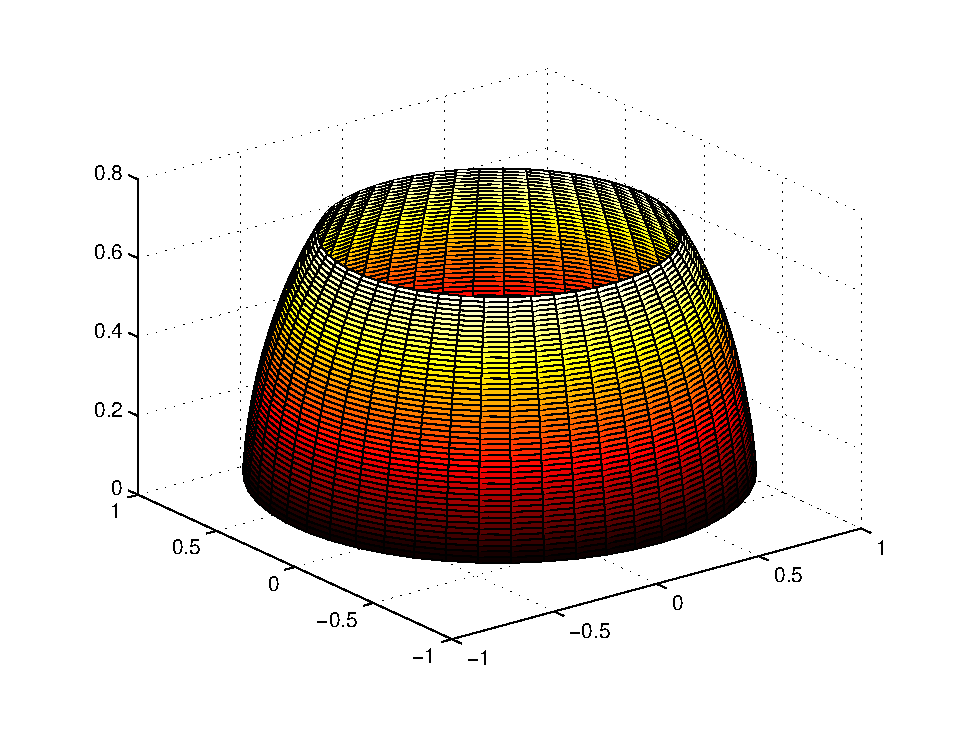
\includegraphics[width=0.75\textwidth]{image.eps}
			\caption{Domínio da aplicação}
			\label{fig:dominio}
		\end{figure}

		\begin{figure}
			\centering
			\begin{subfigure}[b]{0.45\textwidth}
				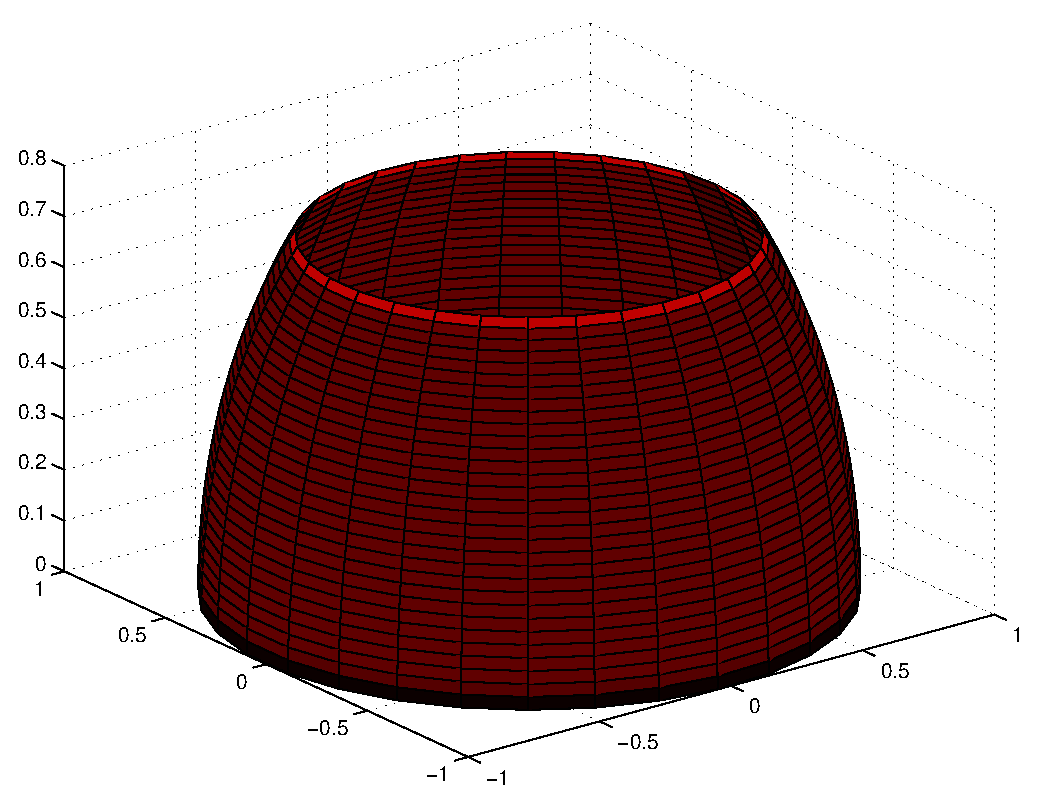
\includegraphics[width=0.9\textwidth]{time-10.eps}
				\caption{10 segundos}
			\end{subfigure}
			\begin{subfigure}[b]{0.45\textwidth}
				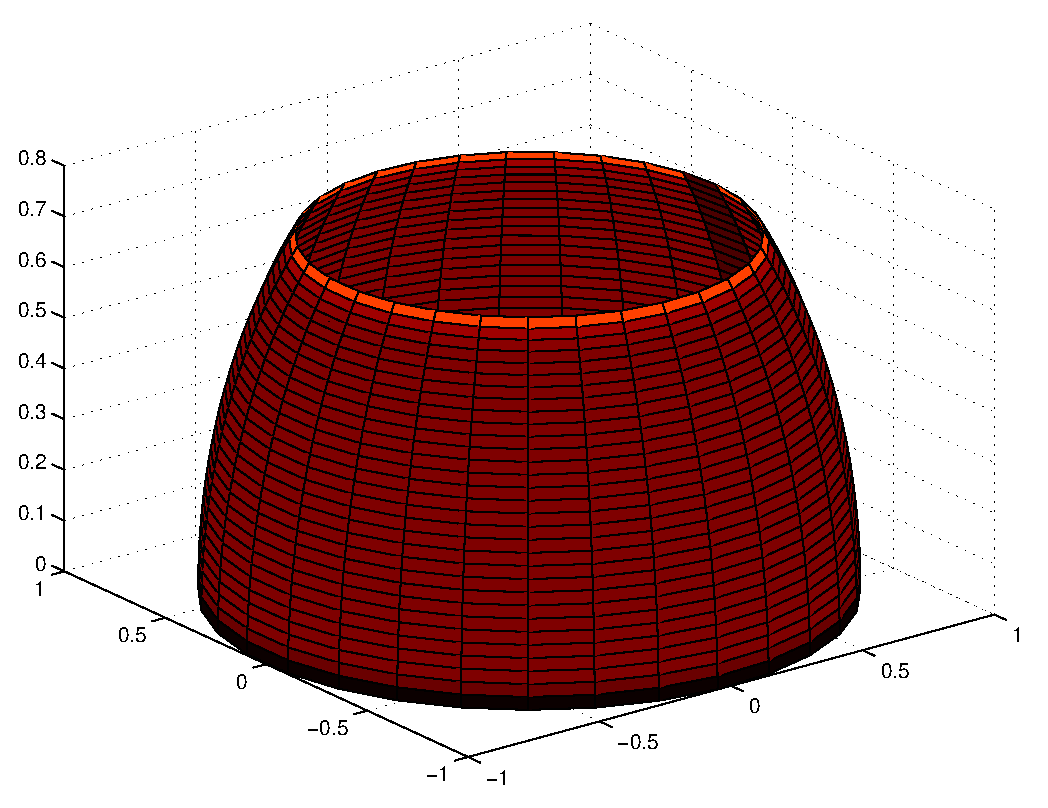
\includegraphics[width=0.9\textwidth]{time-20.eps}
				\caption{20 segundos}
			\end{subfigure}
			\begin{subfigure}[b]{0.45\textwidth}
				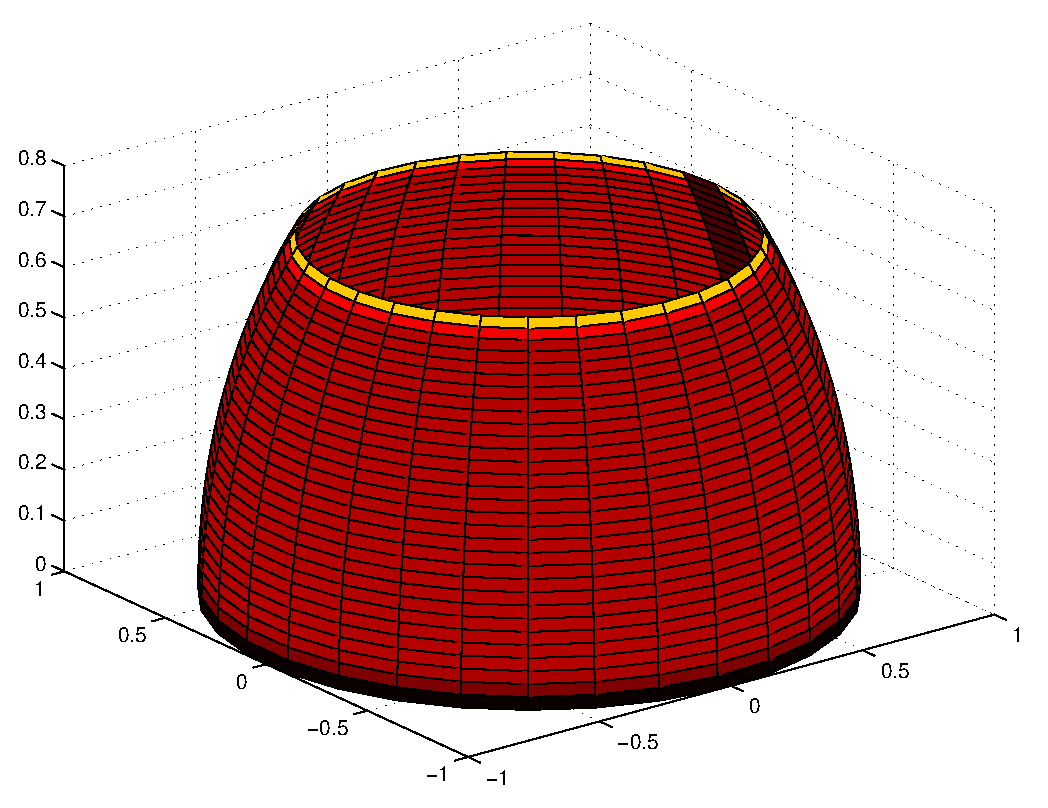
\includegraphics[width=0.9\textwidth]{time-30.eps}
				\caption{30 segundos}
			\end{subfigure}
			\begin{subfigure}[b]{0.45\textwidth}
				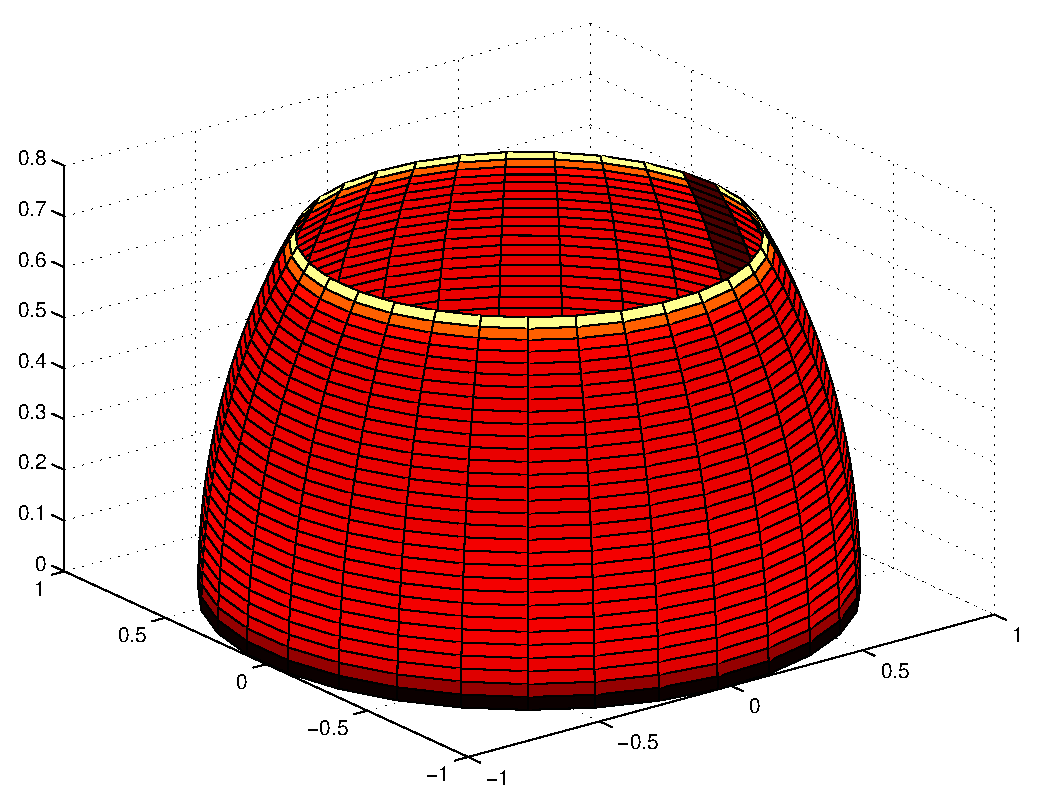
\includegraphics[width=0.9\textwidth]{time-40.eps}
				\caption{40 segundos}
			\end{subfigure}
			\begin{subfigure}[b]{0.45\textwidth}
				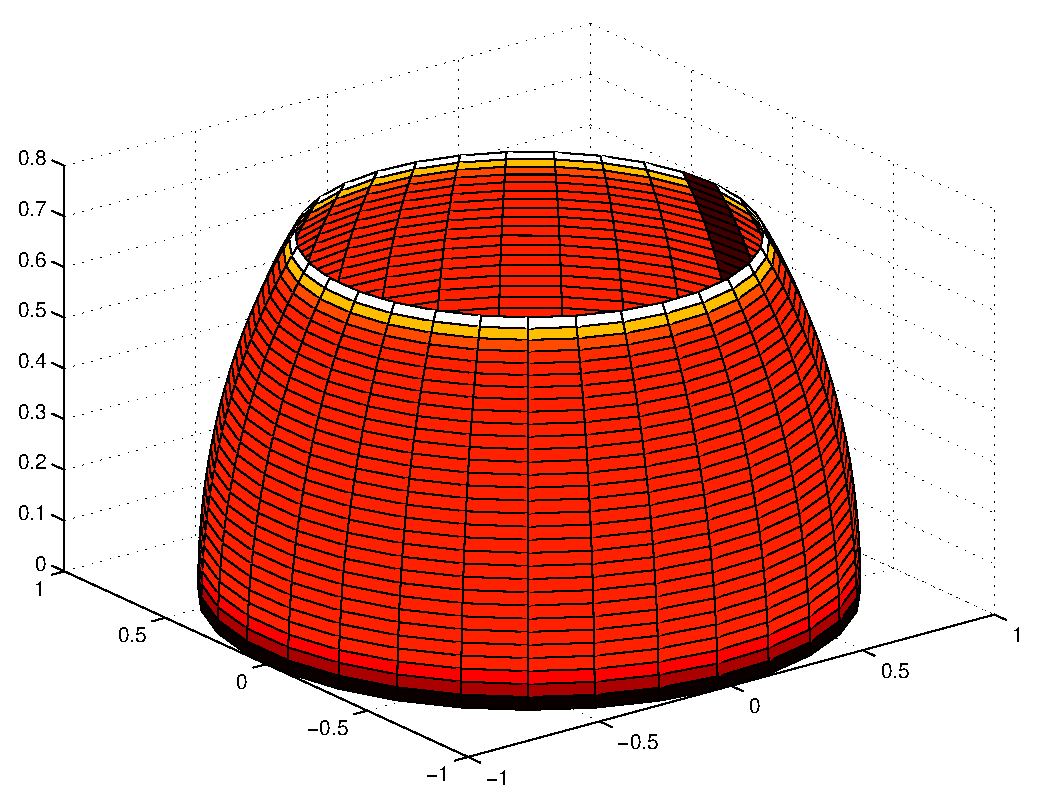
\includegraphics[width=0.9\textwidth]{time-50.eps}
				\caption{50 segundos}
			\end{subfigure}
			\caption{Temperatura ao longo do tempo. Cores mais claras indicam maiores temperaturas}
			\label{fig:simulacao}
		\end{figure}
	\bibliography{refs}
	\bibliographystyle{acm}
\end{document}
